\documentclass[conference]{acmsiggraph}

\usepackage[utf8]{inputenc}  
\usepackage[T1]{fontenc}  

%%% Make the ``BibTeX'' word pretty...

\def\BibTeX{{\rm B\kern-.05em{\sc i\kern-.025em b}\kern-.08em
    T\kern-.1667em\lower.7ex\hbox{E}\kern-.125emX}}

\title{Procedurally Generating Content from Video Stream}

%%% TODO: Mettre les adresses de l'école
%%\author{Guillaume Ambrois\thanks{e-mail:guillaume.ambrois@gmail.com}, Sébastien %%Gaulier\thanks{e-mail:sebastien.gaulier@gmail.com}\\ESGI, Paris}
%%\pdfauthor{Guillaume Ambrois & Sébastien Gaulier}

\author{Anonym}
\pdfauthor{Anonym}

%%\keywords{procedural, computer vision}

\begin{document}

%%% This is the ``teaser'' command, which puts an figure, centered, below 
%%% the title and author information, and above the body of the content.

 \teaser{
   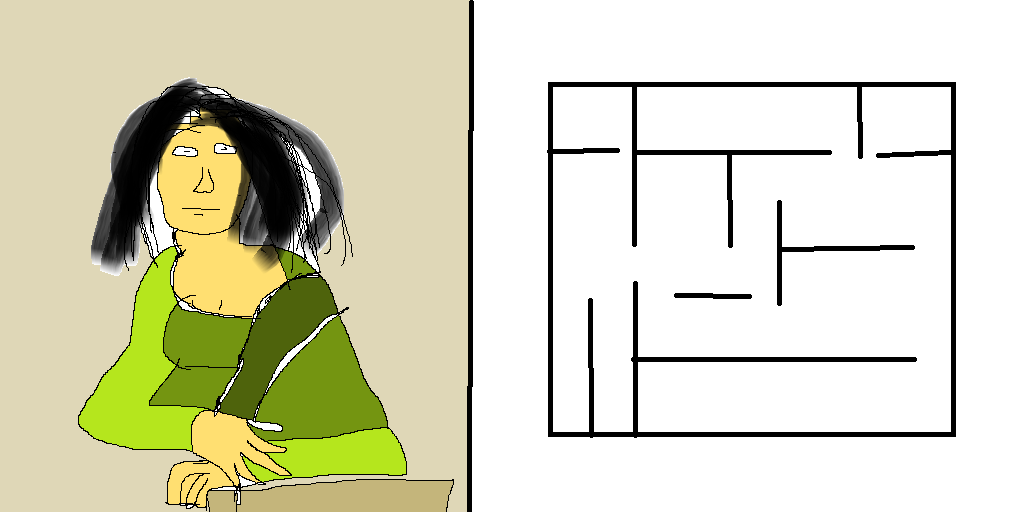
\includegraphics[height=1.5in]{images/sampleteaser}
   \caption{A procedurally generated map from an image}
 }

\maketitle

%% Required for all content. 

\copyrightspace

\section{Introduction}

Over the past years, procedurally generated content has become increasingly popular, especially in video games.

\section{Our design}

In our project, we used Unreal Engine 4 as game engine, and OpenCV 3.1 to process the video from which we want to extract data.

We first had to decide what we wanted to look for in the video.
For this, we considered : 
\begin{itemize}
	\item Moving elements,
	\item Changing colors,
	\item ???,
\end{itemize}

We decided to focus on spotting elements, and their movements, which is the thing the human eye is the best at spotting.

Then, we had to decide what type of content we wanted to procedurally generate using those data.

The game we developed as a proof of concept was a multiplayer arcade game in which you wandered around a maze-ish arena, collecting treasures and battling against other players and IAs.

The content we considered to procedurally generate were :
\begin{itemize}
	\item A level,
	\item An IA behavior (?),
	\item Player capacities,
\end{itemize}

\section{Technical approach}

Firstly, for the sake of simplicity, we used short videos (2 to 3 minutes), with a static point of view.

We process each frame of the video, trying to follow the motion of the elements we're tracking.

\bibliographystyle{acmsiggraph}
\nocite{*}
\bibliography{abstract}
\end{document}
